\documentclass[12pt]{article}

\usepackage[margin=1in]{geometry} 
\usepackage{amsmath,amsthm,amssymb,amsfonts}
\usepackage{graphicx}
\usepackage{listings}
\usepackage{color}
\usepackage{caption}
\usepackage{subcaption}

\definecolor{mygreen}{rgb}{0,0.6,0}
\definecolor{mygray}{rgb}{0.5,0.5,0.5}
\definecolor{mymauve}{rgb}{0.58,0,0.82}

\lstset{basicstyle=\footnotesize ,
tabsize=4,
commentstyle=\color{mygreen},
numbers=left,
numbersep=5pt,
numberstyle=\tiny\color{mygray},
rulecolor=\color{black},
stringstyle=\color{mymauve}}

\graphicspath{{./}}

\begin{document}

\title{CS 5785 Applied Machine Learning, Homework 3}
\author{Wen Guo (wg264), Roger Wang (rw575)}
\maketitle

{\parindent0pt
\section*{Programming Exercises}
\subsection*{Question 1}
\subsubsection*{(a) (b)}
\begin{center}
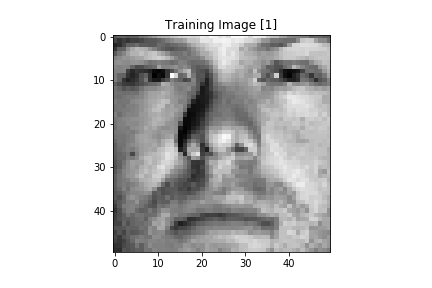
\includegraphics[width=0.8\linewidth]{P1/Training_Image_[1].png}
\end{center}

\begin{center}
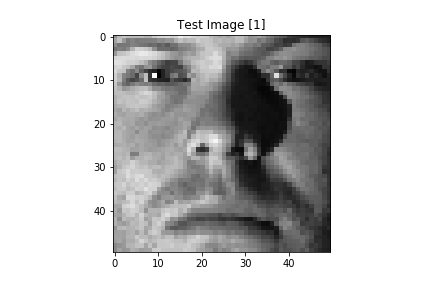
\includegraphics[width=0.8\linewidth]{P1/Test_Image_[1].png}
\end{center}

\subsubsection*{(c)}
The average face: 

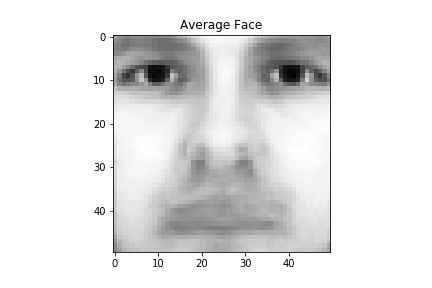
\includegraphics[scale=1]{P1/Average_Face.png}

\subsubsection*{(d)}
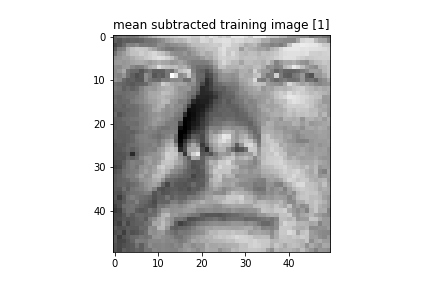
\includegraphics[width=0.8\textwidth]{P1/mean_subtracted_training_image_[1].png}
 
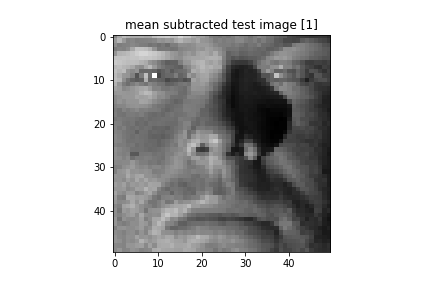
\includegraphics[width=0.8\textwidth]{P1/mean_subtracted_test_image_[1].png}

\subsubsection*{(e)}
These are the top 10 eigenfaces: 
\begin{center}
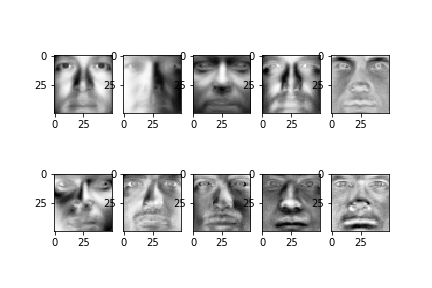
\includegraphics[scale=1]{P1/Top_10_Eigenfaces.png}
\end{center}

\subsubsection*{(f)}
Rank-r approximation error is as follows: 
\begin{center}
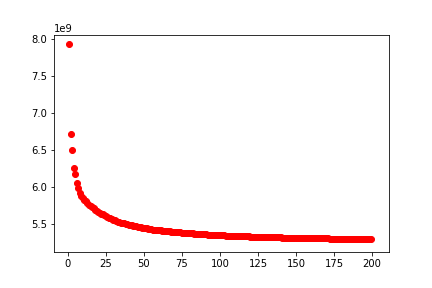
\includegraphics[scale=0.8]{P1/Rank_r_approximation_error.png}
\end{center}

\subsubsection*{(g)}
The following code is used to generate r-dimensional feature matrix: 
\begin{lstlisting}
def feature_generator(matrix_data, matrix_vt, rank_r):
    return np.dot(matrix_data, matrix_vt[0:rank_r,:].transpose())

# generate feature matrix for trainning and test data 
feature_matrix_train = feature_generator(train_data, v_t, 10)
feature_matrix_test = feature_generator(test_data, v_t, 10)
\end{lstlisting}

\subsubsection*{(h)}
According to the following graph, the accuracy stabilize after r is larger than 50. 
\begin{center}
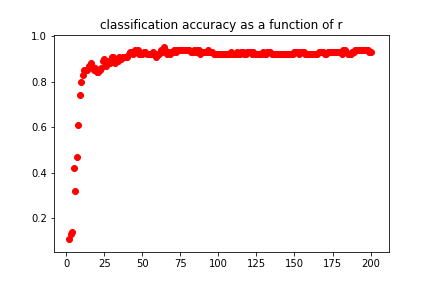
\includegraphics[scale=0.8]{P1/accuracy_over_r.png}
\end{center}

\subsection*{Question 2}
\subsubsection*{(a)}
Choose k = 5. 
\lstinputlisting{P2/doc_K-Mean_top_documents_c5.txt}

\medskip
\lstinputlisting{P2/doc_K-Mean_top_words_c5.txt}

The algorithm has captured five different topics within these documents. The five clusters' topics are approximately biology, news, astronomy, measurement, research. This algorithm may be useful in finding documents with similar appearance of key words. It can be used in search engine to increase search accuracy.

\subsubsection*{(b)}
Choose k = 5.
\lstinputlisting{P2/word_K-Mean_top_words_c5.txt}

\medskip
\lstinputlisting{P2/word_K-Mean_top_documents_c5.txt}

The algorithm cluster words into five categories according to their frequency distribution in documents. The five clusters' seems to have respectively similar frequency in politics, biology, physics, uncommon words, and mutation. This algorithm may be useful in finding words related to a certain topic.

Clustering terms create clusters according to terms distribution among all documents while clustering documents create clusters according to documents similarity. Clustering terms is better in finding similar terms while clustering documents is better in finding similar documents.

\subsection*{Question 3}
\subsubsection*{(a)}
For the K-means algorithm, there are primarily two steps involved. 
\newline
Assignment Step: Assign each observation to the cluster whose mean has the least squared Euclidean distance. This is intuitively the "nearest" mean. Compared with the E-Step of EM algorithm, the K-means assumes that the variance and the size of each cluster are the same.
\newline
Update Step: Based on the assignment above, calculate the new means to be the centroids of the observations in the new clusters. K-means use a hard assignment, which does not capture as much information as the soft assignment used in the E step of EM algorithm. 

\subsubsection*{(b)}
\begin{center}
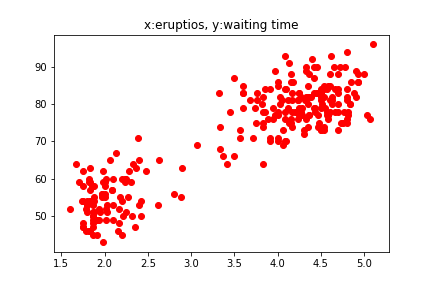
\includegraphics[scale=0.8]{P3/data_on_2D_plane.png}
\end{center}

\subsubsection*{(c)}
The trajectory of the mean vector of cluster 1: 
\begin{center}
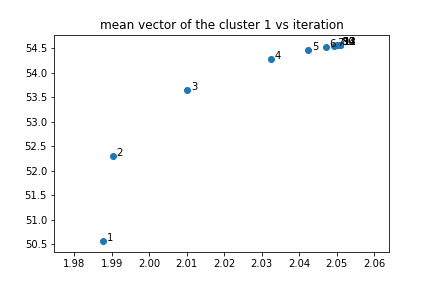
\includegraphics[scale=0.8]{P3/mean_vector_c1.png}
\end{center}

The trajectory of the mean vector of cluster 2: 
\begin{center}
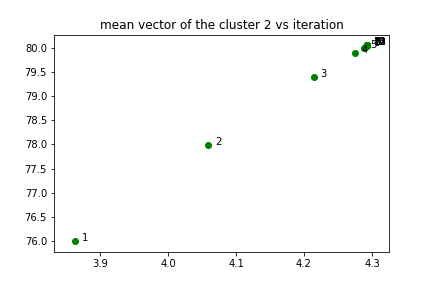
\includegraphics[scale=0.8]{P3/mean_vector_c2.png}
\end{center}

The distribution of total number of iterations:
\begin{center}
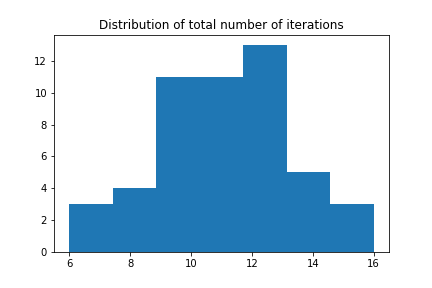
\includegraphics[scale=0.8]{P3/Histogram_iteration_number.png}
\end{center}

\subsubsection*{(d)}
K-means:
\begin{center}
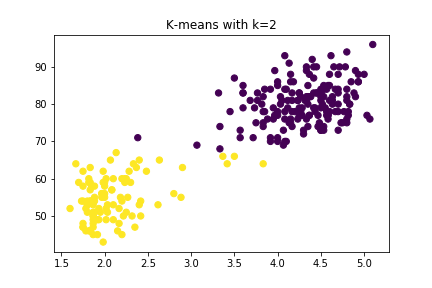
\includegraphics[scale=0.8]{P3/k_means.png}
\end{center}

If we use the labeled data of k-means to initialize the mean and variance of EM, it takes only 10 iterations to converge. However, if we do this randomly, it takes about 12 iterations to converge. 

\subsection*{Question 4}
\subsubsection*{(a)}
i.
Assumptions: there are no extreme values. All variables have equal influence and the differences among samples are based on relative values not their magnitude.

If the variables are not normalized or have extreme values, this assumption can fail.

We can measure using stress. The stress provides a measure of the degree to which the distance between samples in reduced dimensional space (usually 2-dimensions) corresponds with the actual multivariate distance between the samples. Lower stress values indicate greater conformity and therefore are desirable. High stress values indicate that there was no 2-dimensional arrangement of your points that reflect their similarities. The stress values should ideally be less than 0.2.

\medskip
ii.
We did principal component analysis (PCA) on 20 dimensions and showed the percentage of variance explained by each dimension. PCA takes a dataset consisting of a set of tuples representing points in a high-dimensional space and finding the directions along which the tuples line up best. When PCA applies this transformation to the original data, the axis corresponding to the principal eigenvector is the one along which the points are most "spread out" or in other words, maximized data variance. If the total variance is lost a little, then MDS successfully reduces the dimension while maintaining the output quality. In the PCA, 4 dimensions explained over 90\% of variance and 14 dimensions explained over 99\% of variance. 

\medskip
iii.

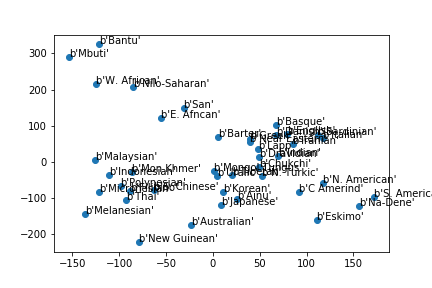
\includegraphics[scale=1]{P4/scatter.png}

\subsubsection*{(b)}
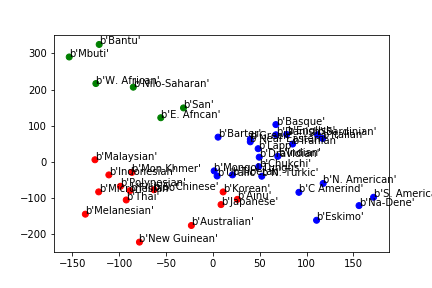
\includegraphics[scale=1]{P4/3-means.png}

I am satisfied with the clustering result. It categorizes languages into African, European + American and Asia. It lost the information about language's position in high dimension space. The x-axis and y-axis don't have any meaning.

\subsubsection*{(c)}

\begin{figure}
\centering
\begin{subfigure}{.49\textwidth}
  \centering
  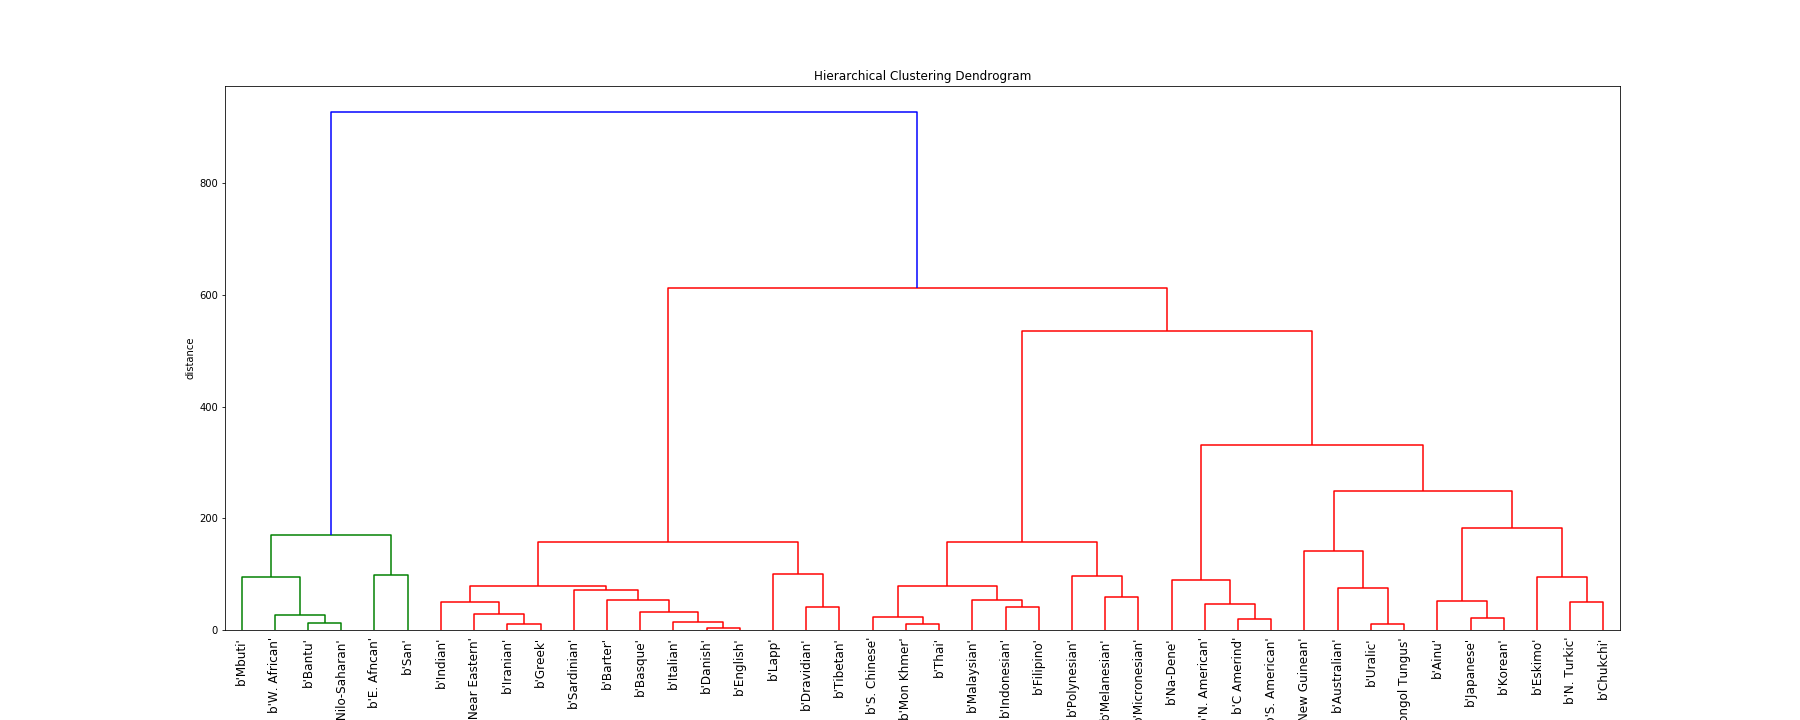
\includegraphics[width=1\linewidth]{P4/dendrogram.png}
  \caption{dendrogram}
\end{subfigure}
\begin{subfigure}{.49\textwidth}
  \centering
  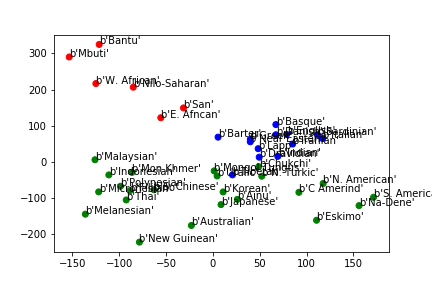
\includegraphics[width=1\linewidth]{P4/hierarchical_3_clusters.png}
  \caption{hierarchical 3 clusters}
\end{subfigure}
\end{figure}
Hierarchical clustering categorizes languages in American continent into Asia language category.

\subsubsection*{(d)}

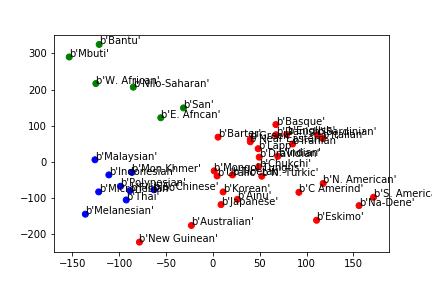
\includegraphics[scale=1]{P4/3-medoids.png}

There are some significant differences. 3-medoids seems less accurate in clustering languages. It has a huge cluster including languages from Asia, Europe, Australia, North America and South America.

\section*{Written Exercises}
\subsection*{Question 1}
\subsubsection*{(a)}
\[
M^TM
=
\begin{bmatrix}
39 & 57 & 60 \\
57 & 118 & 53 \\
60 & 53 & 127
\end{bmatrix},\ 
MM^T
=
\begin{bmatrix}
10 & 9 & 26 & 3 & 26 \\
9 & 62 & 8 & -5 & 85 \\
26 & 8 & 72 & 10 & 50 \\
3 & -5 & 10 & 2 & -1 \\
26 & 85 & 50 & -1 & 138
\end{bmatrix}
\]

\subsubsection*{(b)}
\[
eigenvalues(M^TM)
=
\begin{bmatrix}
214.67 \\
69.33 \\
0.00 \\

\end{bmatrix},\ 
eigenvalues(MM^T)
=
\begin{bmatrix}
214.67 \\
69.33 \\
0.00 \\
0.00 \\
0.00
\end{bmatrix}
\]

\subsubsection*{(c)}
\[
eigenvectors(M^TM)
=
\begin{bmatrix}
0.4262 & -0.0146 & 0.9045 \\
0.6150 & -0.7286 & -0.3015 \\
0.6634 & 0.6848 & -0.3015
\end{bmatrix}\]

\[
eigenvectors(MM^T)
=
\begin{bmatrix}
-0.1649 & 0.2450 & -0.9554 & -0.5400 & -0.7850 \\
-0.4716 & -0.4533 & -0.0348 & -0.6202 & 0.3029 \\
-0.3365 & 0.8294 & 0.2708 & -0.1270 & 0.2857 \\
-0.0033 & 0.1697 & 0.0441 & 0.1602 & 0.4371 \\
-0.7982 & -0.1331 & 0.1037 & 0.5310 & -0.1390
\end{bmatrix}
\]

\subsubsection*{(d)}
$M = U\Sigma V^T$

\medskip
$U=\begin{bmatrix}
-0.1649 & -0.2450 \\
-0.4716 & 0.4533 \\
-0.3365 & -0.8294 \\
-0.0033 & -0.1697 \\
-0.7982 & 0.1331
\end{bmatrix}$, 
$\Sigma=\begin{bmatrix}
14.6516 & 0 \\
0 & 8.3264
\end{bmatrix}$, 
$V=\begin{bmatrix}
-0.4262 & 0.0146 \\
-0.6150 & 0.7286 \\
-0.6634 & -0.6848
\end{bmatrix}$

\subsubsection*{(e)}
$M^*=\begin{bmatrix}
-2.4165 \\
-6.9104 \\
-4.9298 \\
-0.0484 \\
-11.6949
\end{bmatrix}$

\subsection*{Question 2}

$${X^{S}}^{T} X^S = \hat{\Sigma}^{-\frac{1}{2}T}  (X-\bar{X} )^T (X-\bar{X} )  \hat{\Sigma}^{-\frac{1}{2}} = \hat{\Sigma}^{-\frac{1}{2}T} n \hat{\Sigma}  \hat{\Sigma}^{-\frac{1}{2}} = n I
$$

The principle components of $X^S$ is identity matrix. After the standardization, the$X^S$ look like a sphere where the variance in different directions is the same. 

In terms of practical implications of different units of scale, if some variables have a large variance and some small, PCA (maximizing variance) will load on the large variances. For example if you change one variable from km to cm (increasing its variance), it may go from having little impact to dominating the first principle component. If you want your PCA to be independent of such rescaling, standardizing the variables will do that.

}
\end{document}